\documentclass[../Tesi.tex]{subfiles}


\begin{document}
\section{Progettazione}
	\subsection{Architettura ad alto livello}
		\begin{figure}[!h]
			\centering
			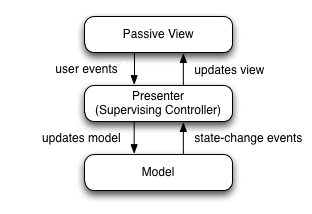
\includegraphics[scale=0.6]{images/mvp}
				\caption{Rappresentazione pattern MVP}
			\label{fig:StrutturaMVP}
		\end{figure}

		L'architettura dell'applicazione segue il pattern architetturale Model-View-Presenter, utilizzato insieme alla dependency injection. Tale scelte, unite ad un uso diffuso di interfacce permettono di ridurre il grado di accoppiamento tra le parti che l'applicazione in modo tale da aumentarne il più possibile l'estensibilità.

		\paragraph*{Model}
		Il model rappresenta i dati che vengono trattati all'interno dell'applicazione. Le classe appartenenti al model rappresentano:
		\begin{itemize}
			\item i dati che vengono salvati in modo persistente nel database presente nel dispositivo in cui è installata l'applicazione;
			\item gli statement che devono essere inviati ad un LRS;
			\item gli oggetti che vengono scambiati tra JavaScript e Android per il tracciamento delle esperienze di un utente;
			\item oggetti che permettono l'accesso a tali dati.
		\end{itemize}
		Nell'applicativo è rappresentato dal package omonimo.

		\paragraph*{Presenter}
		Il presenter si occupa di recuperare i dati del model e passarli alla view per essere mostrati. Esso si occupa inoltre di gestire le richieste della view in seguito ad una interazione con un utente. \\ Nell'applicativo è rappresentato dal package omonimo.

		\paragraph*{View}
		La view si occupa della dell'interfaccia grafica dell'applicazione e di notificare al presenter le interazioni dell'utente, che ha il compito di elaborare. \\ Nell'applicativo è rappresentato dal package omonimo.
	
\end{document}